\section{Distância em $\mathbb R^n$}
A distância entre dois pontos $p, q \in \mathbb R^n$ é dada pela métrica usual (Euclidiana), motivada pelo Teorema de Pitágoras.

\begin{definition}
    Sejam $p, q \in \mathbb R^n$. A \emph{distância (usual, também chamada de Euclidiana)} entre $p$ e $q$ é definida como:
    \begin{equation*}
        d(p, q) = \|p-q\| = \sqrt{(p-q) \cdot (p-q)}=\sqrt{\sum_{i=1}^n (p_i - q_i)^2}.
    \end{equation*}
\end{definition}

Algumas propriedades básicas da distância são as seguintes.
\begin{proposition}
    Sejam $p, q, r \in \mathbb R^n$. Então:
    \begin{enumerate}
        \item $d(p, q) = 0$ se, e somente se, $p=q$.
        \item $d(p, q) = d(q, p)$ (simetria);
        \item $d(p, r) \leq d(p, q) + d(q, r)$ (desigualdade triangular).
    \end{enumerate}
\end{proposition}
\begin{proof}
    Vamos verificar cada uma das propriedades.
    \begin{enumerate}
        \item Dados $p$ e $q$, temos que $d(p, q) = 0$ se, e somente se, $\|p-q\|=0$, o que ocorre se, e somente se, $p-q=0$, ou seja, $p=q$.
        \item Temos que $d(p, q) = \|p-q\| = |-1|\|p-q\| = \|q-p\| = d(q, p)$.
        \item Temos que:
        \begin{align*}
            d(p, r) &= \|p-r\| = \|p-q+q-r\| \\
            &\leq \|p-q\| + \|q-r\| = d(p, q) + d(q, r).
        \end{align*}
    \end{enumerate}
\end{proof}

A seguir, definiremos generalizações da noção de intervalo aberto de $\mathbb R$, conceitos essenciais para o futuro estudo de limite, continuidade e diferenciabilidade em $\mathbb R^n$.

\begin{definition}
    Sejam $p \in \mathbb R^n$ e $r>0$. A \emph{bola aberta} de centro $p$ e raio $r$ é o conjunto:
    \begin{equation*}
        B(p, r) = \{q \in \mathbb R^n : d(p, q) < r\}.
    \end{equation*}
    A \emph{bola fechada} de centro $p$ e raio $r$ é o conjunto:
    \begin{equation*}
        \overline B(p, r) = \{q \in \mathbb R^n : d(p, q) \leq r\}.
    \end{equation*}
\end{definition}

Uma bola aberta de raio $r$ centrada em $p$ é ilustrada abaixo.

\begin{figure}[ht]
    \centering
    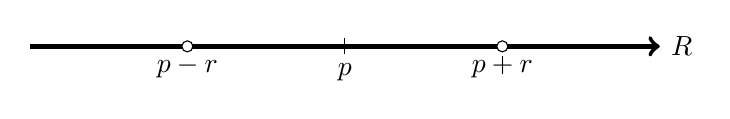
\begin{tikzpicture}
        % Eixo real
        \draw[->,ultra thick] (-4,0)--(4,0) node[right]{$\mathbb R$};
        % Intervalo aberto (p-r, p+r)
        \draw[thick] (-2,0) -- (2,0);
        % Pontos abertos nas extremidades
        \draw[fill=white] (-2,0) circle (2pt) node[below]{$p - r$};
        \draw[fill=white] (2,0) circle (2pt) node[below]{$p + r$};
        % Centro p
        \draw (0,0.1) -- (0,-0.1) node[below]{$p$};
    \end{tikzpicture}
    \caption{Bola aberta de centro $p$ e raio $r$ em $\mathbb R$.}
\end{figure}
\begin{figure}[ht]
    \centering
    \begin{tikzpicture}
    \draw[->,ultra thick] (-4,0)--(4,0) node[right]{$x$};
    \draw[->,ultra thick] (0,-4)--(0,4) node[above]{$y$};
    % Centro da bola
    \filldraw[black] (2,2) circle (2pt);
    \node[below right] at (2,2) {$p$};
    % Raio da bola
    \draw[dashed] (2,2) circle (1.5);
    % Desenho do raio da bola
    \draw[-,thick] (2,2) -- (3.5,2) node[above right]{$r$};
    \end{tikzpicture}
    \caption{Bola aberta de centro $p$ e raio $r$ em $\mathbb R^2$.}
\end{figure}
